
\documentclass{article}

\usepackage{graphicx}
\usepackage{apacite}
\usepackage{natbib}
\usepackage[linktocpage]{hyperref}
\usepackage[fleqn]{amsmath}
\usepackage{mathtools}
\usepackage{amsthm}
\usepackage{amssymb}
\usepackage{verbatim}
\usepackage{lineno}
\usepackage{bm}
\usepackage{color}

\allowdisplaybreaks
\linenumbers

\DeclarePairedDelimiterX{\inp}[2]{\langle}{\rangle}{#1, #2}

\newtheorem{malkinsTheorem}{Theorem}
\newtheorem{simplification1}{Lemma}
\newtheorem{simplification1.1}{Lemma}

\begin{document}

\title{Verification of Malkin's theorem and report of problem in Figure~10-26,
panel $I_{Na}+I_K$-model (Class 2), and in Figure~10-30a, of \citet{izhikevich07}}
\author{Joaqu\'{i}n Rapela\thanks{rapela@ucsd.edu}}
\maketitle

\tableofcontents

\section{Introduction}

Below I state Malkin's theorem, following Theorem 9.2 in
\citet{hoppensteadtAndIzhikevich97} (Section~\ref{sec:malkinsTheorem}),
present two succesive simplification and one example of this theorem
(Section~\ref{sec:malkinsTheormeSimplificationsAndExample}),
%
report a problem in Figure~10-26, panel $I_{Na}+I_K$-model (Class 2), and in
Figure~10-30a, of
\citet{izhikevich07} (Section~\ref{sec:problemInIzhikevich}), and verify the
validity of Malkin's theorem and that of the repoted problem
(Section~\ref{sec:verificationMalkinsTheorem}).

\section{Malkin's Theorem}
\label{sec:malkinsTheorem}

The following statement of Malkin's theorem is a modification of that given in
Theorem 9.2 of \citet{hoppensteadtAndIzhikevich97}. 

\begin{malkinsTheorem}

Let $\bm{X}_i(t)\in\Re^m, i=1, \ldots, n,$ be weakly-connected m-dimensional dynamical
systems

\begin{align}
\dot{\bm{X}}_i=F_i(\bm{X}_i)+\epsilon G_i(\bm{X})
\label{eq:xiDot}
\end{align}

\noindent where
$\bm{X}(t_1,\ldots,t_n)=(\bm{X}_1(t_1),\ldots,\bm{X}_n(t_n))\in\Re^{m\times n}$. Assume that
each uncoupled system

\begin{align}
\dot{\bm{X}}_i=F_i(\bm{X}_i)
\end{align}

\noindent is on a limit cycle of length $T$ parametrized by
$\gamma_i: S^1\rightarrow \Re^m$, $\gamma_i(\theta_i)=\bm{X}_i(\theta_i)$.
Define
$\gamma(\theta_1,\ldots,\theta_n)=(\gamma_1(\theta_1),\ldots,\gamma_n(\theta_n))$,
and let $\varphi_i$ be the phase deviation of $X_i$ (i.e.,
$\theta_i=(t+\varphi_i)\;\bmod\;T$). Then

\begin{align}
\dot{\varphi}_i=H_i(\bm{\varphi}-\varphi_i,\epsilon)
\label{eq:phiiDot}
\end{align}

\noindent with
$\bm{\varphi}-\varphi_i=(\varphi_1-\varphi_i,\ldots,\varphi_n-\varphi_i)$, and

\begin{align}
H_i(\bm{\varphi}-\varphi_i,0)&=\frac{1}{T}\int_{0}^{T}Q_i(\theta)^TG_i(\gamma(\theta+\bm{\varphi}-\varphi_i))\;d\theta
\label{eq:Hi}
\end{align}

\noindent where $Q_i(\theta)$ is the solution of

\begin{align}
\dot{Q}_i(\theta)&=(DF_i(\gamma_i(\theta)))^TQ_i(\theta)
\end{align}

\noindent statisfying the normalization condition

\begin{align}
Q_i(0)^T&DF_i(\gamma_i(0)))=1
\end{align}

\end{malkinsTheorem}

\section{Two succesive simplifications and one example of Malkin's theorem}
\label{sec:malkinsTheormeSimplificationsAndExample}

\subsection*{Simplification 1}

\begin{simplification1}

If in Eq.~\ref{eq:xiDot} the coupling term of oscillator $i$ ($G_i$) is the
sum of coupling terms with other oscillator ($g_{ij}$) and a self coupling
term ($g_{ii}$):

\begin{align}
G_i(X(t))=\sum_{j=1}^n g_{ij}(X_i(t), X_j(t))
\label{eq:restrictedGi}
\end{align}

\noindent then

\begin{align}
\dot{\varphi_i}=\omega_i+\epsilon\sum_{\substack{j=1\\j\neq i}}^n H_{ij}(\varphi_j-\varphi_i,0)
\label{eq:phiiDotSimplified}
\end{align}

\noindent with

\begin{align}
H_{ij}(\varphi_j-\varphi_i,0)=\frac{1}{T}\int_0^TQ_i(\theta)^Tg_{ij}(\gamma_i(\theta),\gamma_j(\theta+\varphi_j-\varphi_i))\;d\theta
\label{eq:Hij}
\end{align}

\noindent and

\begin{align}
w_i=H_{ii}(0,0)
\label{eq:wi}
\end{align}

\end{simplification1}

\begin{proof}
\noindent Using Eq.~\ref{eq:restrictedGi} in Eq.~\ref{eq:Hi} we have

\begin{align}
H_i(\bm{\varphi}-\varphi_i,0)&=\sum_{j=1}^n\frac{1}{T}\int_0^TQ_i(\theta)^Tg_{ij}(\gamma_i(\theta),\gamma_j(\theta+\varphi_j-\varphi_i))\;d\theta\nonumber\\
&=\sum_{j=1}^nH_{ij}(\varphi_j-\varphi_i,0)
\label{eq:HiAsaSumHij}
\end{align}

\noindent Then 

\begin{align}
\dot{\varphi_i}&=H_i(\bm{\varphi}-\varphi_i,\epsilon)=\epsilon
H_i(\bm{\varphi}-\varphi_i,0)=\epsilon\sum_{j=1}^nH_{ij}(\varphi_j-\varphi_i,0)\nonumber\\
&=\epsilon H_{ii}(0,0)+\epsilon\sum_{\substack{j=1\\j\neq i}}^n
H_{ij}(\varphi_j-\varphi_i,0)\nonumber\\
&=\omega_i+\epsilon\sum_{\substack{j=1\\j\neq i}}^n H_{ij}(\varphi_j-\varphi_i,0)
\label{eq:phiiDotSimplification1}
\end{align}

The first equality in Eq.~\ref{eq:phiiDotSimplification1} follows from
Malkin's theorem (Eq.~\ref{eq:phiiDot}), 
%
I cannot understand why the second equality holds, 
%
the third equality follows from Eq.~\ref{eq:HiAsaSumHij}, the right-hand
side of fourth inequality separates the constant and non-constant terms in the
left-hand side, and the last equality uses Eq.~\ref{eq:wi}.

\end{proof}

\subsection*{Simplification 1.1}

\begin{simplification1.1}
If we take $n=2$ in Eq.~\ref{eq:phiiDotSimplified} we obtain

\begin{align}
\dot{\chi}=\epsilon\omega+\epsilon G(\chi)
\label{eq:chiDot}
\end{align}

\noindent where

\begin{align}
\chi&=\varphi_2-\varphi_1\label{eq:chi}\\
\omega&=\omega_2-\omega_1\label{eq:omega}\\
G(\chi)&=H_{21}(-\chi)-H_{12}(\chi)\label{eq:G}
\end{align}

\end{simplification1.1}

\begin{proof}
Taking $i=1$ and $i=2$ in Eq.~\ref{eq:phiiDotSimplified} we obtain

\begin{align}
\varphi_1(t)&=\epsilon\omega_1+\epsilon H_{12}(\varphi_2(t)-\varphi_1(t),0)\label{eq:phi1ProofSimplification1.1}\\
\varphi_2(t)&=\epsilon\omega_2+\epsilon H_{21}(\varphi_1(t)-\varphi_2(t),0)\label{eq:phi2ProofSimplification1.1}
\end{align}

Subtracting Eq.~\ref{eq:phi1ProofSimplification1.1} from
Eq.~\ref{eq:phi2ProofSimplification1.1} and using Eqs.~\ref{eq:chi}-\ref{eq:G}
we obtain Eq.~\ref{eq:chiDot}.

\end{proof}

\paragraph{Note 1} $\chi$ is a fixed point of Eq.~\ref{eq:chiDot} if and only
if $G(\chi)=-\omega$ (Figure~\ref{fig:fixedPoints}).

\begin{figure}
\begin{center}
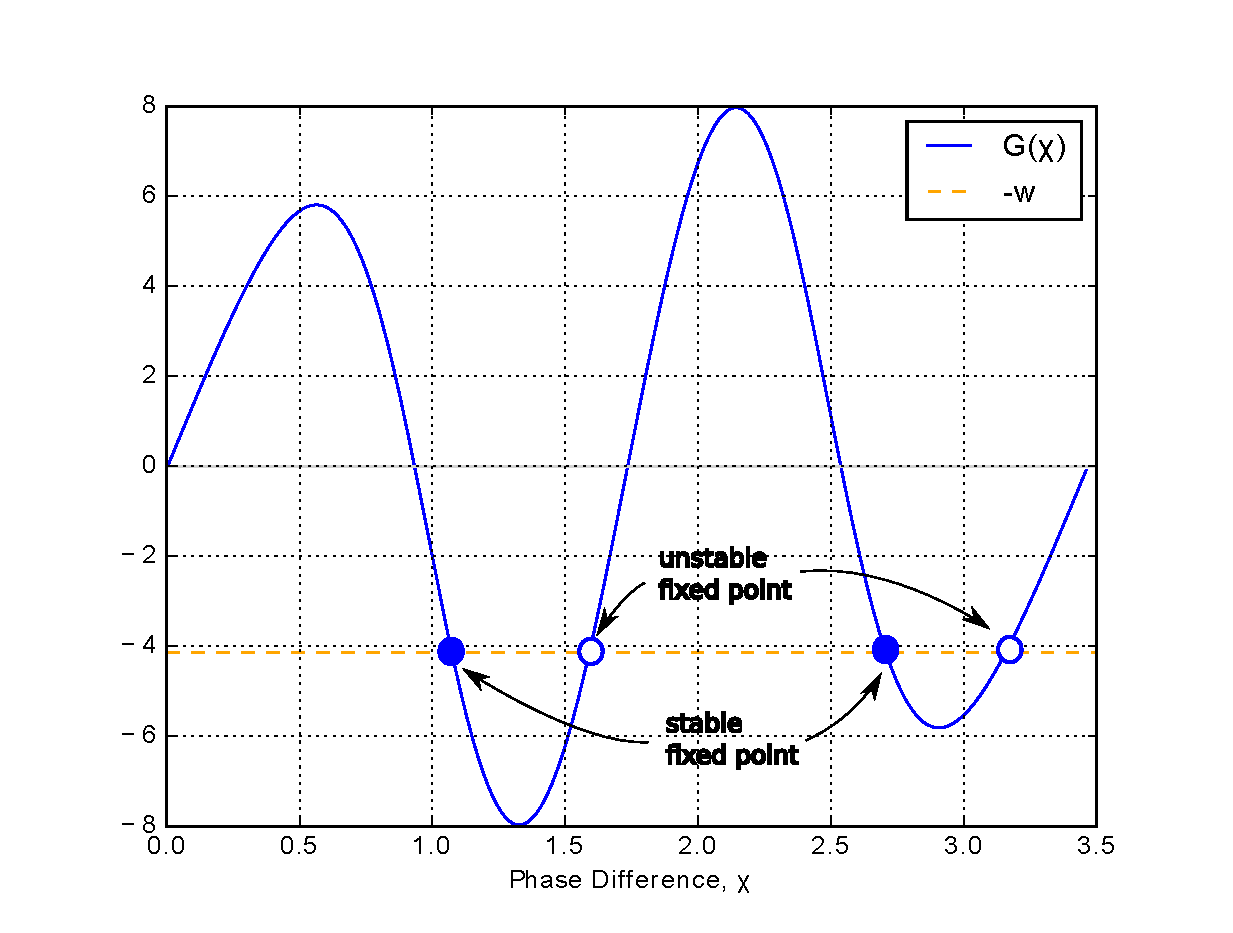
\includegraphics[width=4in]{figures/fig10_30INapIKLowThresholdWithSelfCouplingStrength-3.00I035.00-annotated.eps}
\end{center}
\caption{Fixed points of phase model in Eq.~\ref{eq:chiDot}.}
\label{fig:fixedPoints}
\end{figure}

\paragraph{Note 2} If oscillators are not self coupled (i.e.,
$g_{ii}(\gamma_i(\theta),\gamma_i(\theta))=0\;\forall i$), then (from
Eq.~\ref{eq:Hij}) $H_{ii}=0\;\forall i$, then (from Eq.~\ref{eq:wi})
$w_i=0\;\forall i$, and then the fixed points of Eq~\ref{eq:chiDot} are the
zero crossings of $G(\chi)$.

\subsection*{Example}

This example attempts to replicate that in Figure~10.26 of
\citet{izhikevich07}. 
%%
I simulated two two-dimensional low-threshold INap+IK models of
neurons~\citep{izhikevich07} with the same parameters used in
Figure~10.26 of \citet{izhikevich07}. The two models shared the same
parameters (as given in Figure~4.1b of \citet{izhikevich07} and repeated for
reproducibility in Table~\ref{table:INapIKParams}), but had different initial
conditions (Table~\ref{table:initialConditions}). The input current to both
models was such that when uncoupled these models were on a stable limit cycle
(I=35, INap+IK (Class 2) model on Figure~10.3 of \citet{izhikevich07} and blue
traces in Figure~\ref{fig:neuronsInLimitCycle}). These models were weakly
coulpled with gap junctions (Eq.~\ref{eq:crossCoupling}), and the coupling strength was weak enough
($\epsilon=0.003$ in Eq.~\ref{eq:xiDot}) so that
the coupled models
remained on the uncoupled stable limit cylce (red traces in
Figure~\ref{fig:neuronsInLimitCycle}). The model of neuron~1
(Eq.~\ref{eq:selfCoupling1}), but not that of
neuron~2 (Eq.~\ref{eq:selfCoupling2}), was self coupled, and below we vary the
self-coupling strength of neuron~1 ($s$ in Eq.~\ref{eq:selfCoupling1}) to
obtain different patterns of synchronization between neurons~1 and~2.

\begin{align}
g_{ij}(\gamma_i(\theta),\gamma_j(\theta))=\left[\begin{array}{c}
                                                  \gamma_j(\theta)[0]-\gamma_i(\theta)[0]\\
                                                  0
                                                \end{array}\right], i\ne j
\label{eq:crossCoupling}
\end{align}

\begin{align}
g_{11}(\gamma_1(\theta),\gamma_1(\theta))&=\left[\begin{array}{c}
                                                   s\times \gamma_1(\theta)[0]\\
                                                   0
                                                 \end{array}\right]\label{eq:selfCoupling1}\\
g_{11}(\gamma_2(\theta),\gamma_2(\theta))&=0\label{eq:selfCoupling2}
\end{align}

\begin{table}
\begin{center}
\begin{tabular}{|l|c|}\hline
\multicolumn{1}{|c}{Name} & \multicolumn{1}{|c|}{Value}\\ \hline \hline
$C$ & 1.0 \\ \hline
$g_L$ & 8.0 \\ \hline
$e_L$ & -78.0 \\ \hline
$g_{NA}$ & 20.0 \\ \hline
$e_{NA}$ & 60.0 \\ \hline
$g_{K}$ & 10.0 \\ \hline
$e_{K}$ & -90.0 \\ \hline
$mV_{1/2}$ & -90.0 \\ \hline
$mk$ & 15.0 \\ \hline
$nV_{1/2}$ & -45.0 \\ \hline
$nk$ & 5.0 \\ \hline
$\tau$ & 1.0 \\ \hline
\end{tabular}
\end{center}
\caption{Parameters for the the two INap+IK models of neurons, repeated from
Figure~4.1b in \citet{izhikevich07}.}
\label{table:INapIKParams}
\end{table}

\begin{table}
\begin{center}
\begin{tabular}{|c|l|c|}\hline
\multicolumn{1}{|c}{Neuron} & \multicolumn{1}{|c}{Name} & \multicolumn{1}{|c|}{Value}\\ \hline \hline
1 & $V_0$ & -26.30 \\ \hline
1 & $n_0$ & 0.50 \\ \hline
2 & $V_0$ & -65.01 \\ \hline
2 & $n_0$ & 0.16 \\ \hline
\end{tabular}
\end{center}
\caption{Initial conditions for voltages, $V$, and activation gates, $n$, of the
simulated INap+IK models of neurons.}
\label{table:initialConditions}
\end{table}

\begin{figure}
\begin{center}
\includegraphics[width=4.00in]{../../ch10/figures/phaseSpaceNeuron0WCoupledINIKLowThresholdWithSelfCouplingStrength-7.50I035.00Epsilon0.003000CouplingStartTime100.44V00-26.30N000.50.eps}
\includegraphics[width=4.00in]{../../ch10/figures/phaseSpaceNeuron1WCoupledINIKLowThresholdWithSelfCouplingStrength-7.50I035.00Epsilon0.003000CouplingStartTime100.44V00-65.01N000.16.eps}

\caption{Phase space of the two simulated INap+IK neurons.}

\label{fig:neuronsInLimitCycle}
\end{center}
\end{figure} 

\section{Problem in Figure~10-26 of \citet{izhikevich07}}
\label{sec:problemInIzhikevich}

As demonstrated in the next section, the plot of functions $H_{ij}$ and
$G(\chi)$ in Figure~10-26 of \citet{izhikevich07} are inverted. The correct
figure is Fig.~\ref{fig:correctFig10-26INapIKLowThresholdI035.esp}.

\begin{figure}
\begin{center}
\includegraphics[width=4.00in]{../../ch10/figures/fig10_26INapIKLowThresholdI035.00.eps}

\caption{}

\label{fig:correctFig10-26INapIKLowThresholdI035.esp}
\end{center}
\end{figure} 

\section{Verification of Malkin's Theorem}
\label{sec:verificationMalkinsTheorem}

\begin{figure}
\begin{center}
\includegraphics[width=4.00in]{../../ch10/figures/fig10_30INapIKLowThresholdWithSelfCouplingStrength-3.00I035.00.eps}

\caption{}

\label{fig:gSelfCoupling-3.0} 
\end{center}
\end{figure} 

\begin{figure}
\begin{center}
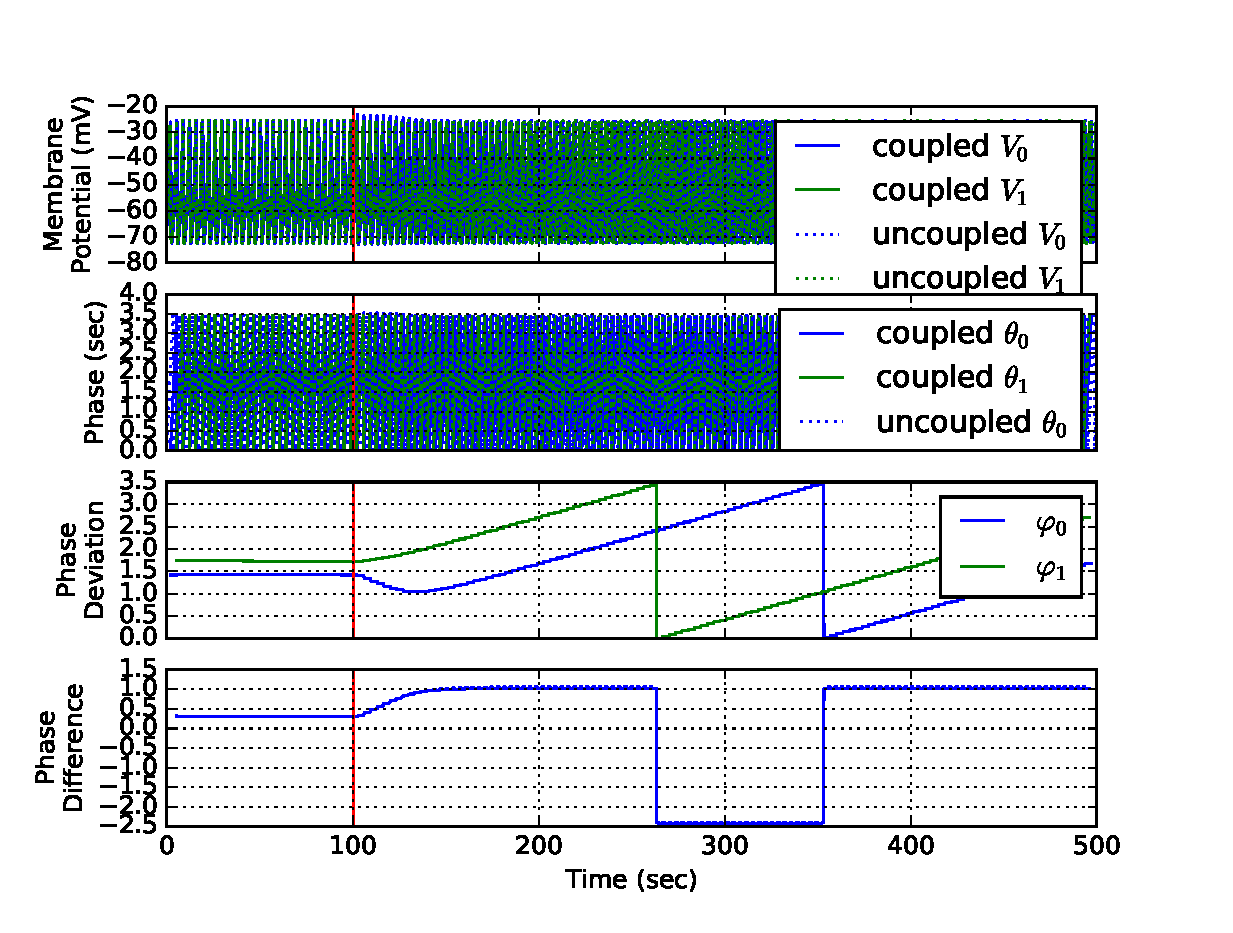
\includegraphics[width=5.50in]{../../ch10/figures/fig10_25INapIKLowThresholdWithSelfCouplingStrength-3.00I035.00Epsilon0.003000CouplingStart100.44V00-67.42N000.20V01-65.01N010.16.eps}

\caption{}

\label{fig:selfCoupling-3.0_lowerConvergence}
\end{center}
\end{figure} 

\begin{figure}
\begin{center}
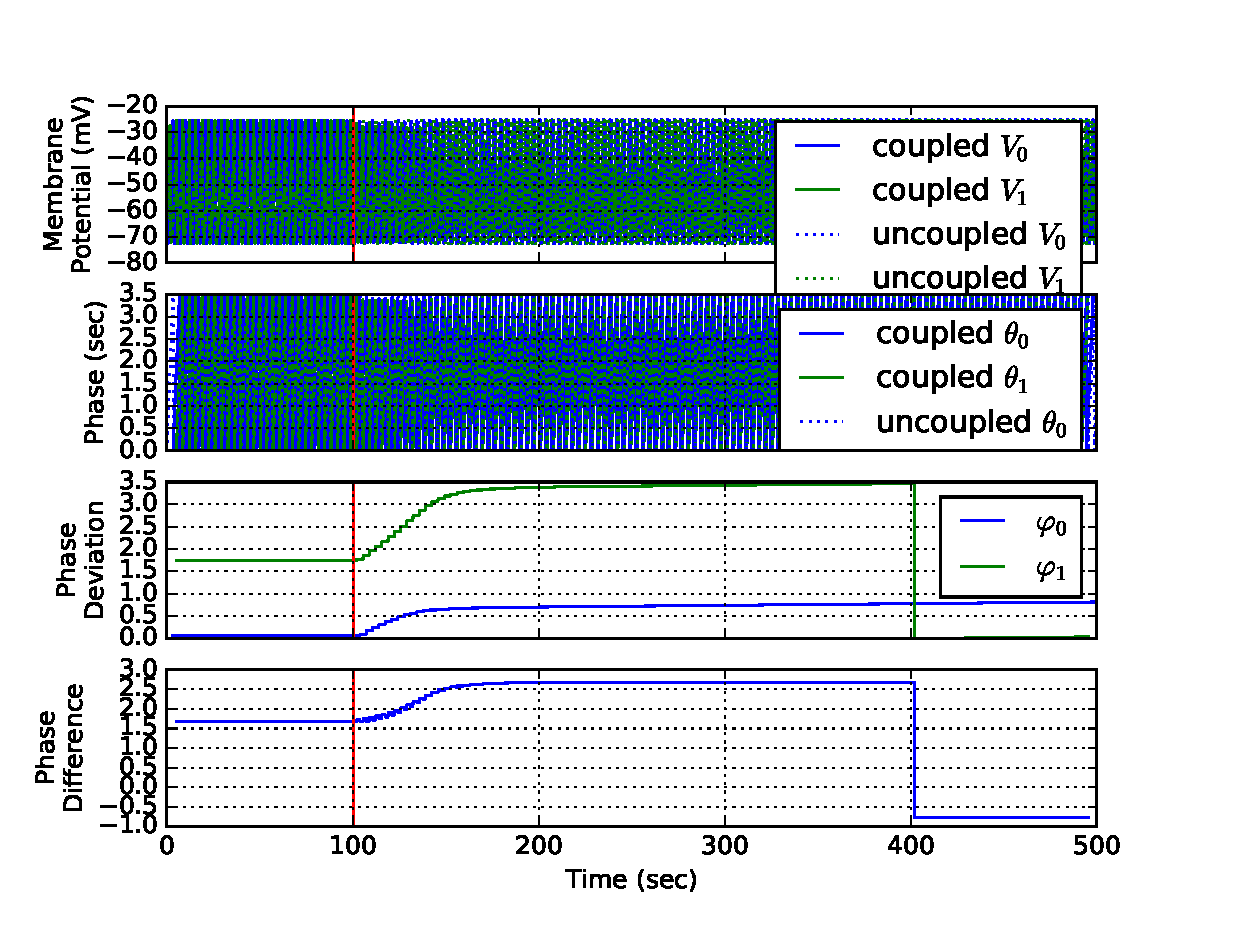
\includegraphics[width=5.50in]{../../ch10/figures/fig10_25INapIKLowThresholdWithSelfCouplingStrength-3.00I035.00Epsilon0.003000CouplingStart100.44V00-26.30N000.50V01-65.01N010.16.eps}

\caption{}

\label{fig:selfCoupling-3.0_upperConvergence}
\end{center}
\end{figure} 

\begin{figure}
\begin{center}
\includegraphics[width=4.00in]{../../ch10/figures/fig10_30INapIKLowThresholdWithSelfCouplingStrength-5.50I035.00.eps}
\includegraphics[width=5.50in]{../../ch10/figures/fig10_25INapIKLowThresholdWithSelfCouplingStrength-5.50I035.00Epsilon0.003000CouplingStart100.44V00-26.30N000.50V01-65.01N010.16.eps}

\caption{}

\label{fig:selfCoupling-5.5} 
\end{center}
\end{figure} 

\begin{figure}
\begin{center}
\includegraphics[width=4.00in]{../../ch10/figures/fig10_30INapIKLowThresholdWithSelfCouplingStrength-7.50I035.00.eps}
\includegraphics[width=5.50in]{../../ch10/figures/fig10_25INapIKLowThresholdWithSelfCouplingStrength-7.50I035.00Epsilon0.003000CouplingStart100.44V00-26.30N000.50V01-65.01N010.16.eps}

\caption{}

\label{fig:selfCoupling-7.5} 
\end{center}
\end{figure} 

\bibliographystyle{apacite}
\bibliography{dynamicalSystems}

\end{document}
